
\subsection{The Filesystem}

We model a working filesystem
using a function $\FS$ with a set of nodes (filesystem paths) $\setn$ as its domain,
and a set of possible contents or values $\setv$ as its codomain.
\begin{mydef}[Filesystems, $\setn$, $\setv$, $\setfs$ and $\empt$]
\[ \FS: \setn \rightarrow \setv \]
In our model, $\setn$ 
serves as a namespace or ``skeleton'' for the filesystem.
It contains all possible nodes, including the ones 
where the file system contains no file or directory,
where in our model $\FS$ has a special value, $\empt\in\setv$.
We write $\setfs$ for the set of filesystems over $\setn$.
\end{mydef}

There is an ancestor / descendant relation defined over the nodes,
which arranges them in a (disjoint) union of rooted directed trees,
and which can be derived from the following $\parent$ function.
Tao et al. \cite{TSR} describe a similar filesystem model, although
they also model inodes and restrict the filesystem to just a single tree.
\begin{mydef}[$\parent$]
The partial function $\parent:\setn\nrightarrow\setn$
returns the parent node of $n$,
and is undefined if $n$ is the root of a tree.
\end{mydef}

\begin{mydef}[$\descendant$, $\descendantEq$]
On $\setn$ the \emph{ancestor / descendant} relation $\descendant$ is the
strict partial ordering determined by the $\parent$ function.
We write $n\descendant m$ if $n$ is the ancestor of $m$,
that is, $n=\parent^i(m)$ for some integer $i\ge 1$.
% or the path name of $n$ is an initial segment of that of $m$. 
We write $n\descendantEq m$ if $n\descendant m$ or $n=m$.
\end{mydef}

\begin{mydef}[$n\unrel m$]
We write $n\unrel m$, or $n$ and $m$ are \emph{incomparable}
iff $n\not\descendantEq m$ and $n\not\ancestorEq m$;
that is, incomparable nodes are on different branches or on different trees.
% none of the path names describing their location is an initial segment of the other.
\end{mydef}

Every working filesystem has a so-called \emph{tree property}, which means that
if the filesystem is not empty at a node, and the node has a parent,
then there must be a directory at the parent node.
To model this, we differentiate between files, directories, and the
empty value in $\setv$, and introduce the equivalence relation
$\typeeq$.

\begin{mydef}[Equivalence by type: $\typeeq$]
We write $v_1\typeeq v_2$ for $v_1,v_2\in\setv$ iff $v_1$ and $v_2$ are both files,
are both directories, or are both $\empt$.
% In other words, if $\setf$ is the set of file values and $\setd$ is the set of directories, then
% with $\{\empt\}$ they form a partition of $\setv$:
% \[ \setv/{\typeeq} = \{\setd,\setf,\{\empt\}\}. \]
\end{mydef}

As usual, we write $[v]$ for the equivalence class of $v$, which represents its type.
We also consider metadata to be part of the values in $\setv$.

The formal definition of the tree property is therefore
\begin{mydef}[Tree property]
\[ \forall n\in\setn, \FS\in\setfs: \FS(n) \neq \empt \Longrightarrow \FS(\parent(n)) \in \setd \]
where $\parent(n)$ is defined, and where $\setd\subset\setv$ is the set of directories.
\end{mydef}

To avoid the proliferation of edge cases, we will furthermore suppose that
$|\setd|=1$, that is, apart from their location, all directories are equal;
and use $\vald$ to denote the single value of the directory type.
In appendix TODO we describe why it can be a sensible choice
for actual synchronizers, and we also present an encoding that makes it possible
to extend our results to the $|\setd|>1$ case.

%% TODO
% % To model this, in $\setv$ we select another special value
% % to represent directories, as we assume that apart from their location
% % in the filesystem, all directories are equal.
% % We do this because, as Bill Zissimopoulos pointed 
% % out \cite{BZ},
% % we often do not want to consider metadata stored in
% % directories (e.g. permission settings) during synchronization,
% % as these are not generally understood well by users,
% % and, if needed, conflict resolution on these settings can be easily automated.
% % We will also see that this assumption makes it possible
% % to define a maximal reconciliation algorithm.


% This means that as we move down from the root of a tree of nodes,
% the types of values we encounter in the filesystem can only change according to the
% transition diagram in \cref{fig_transition}, from directories ($\cchard$) to files ($\ccharf$)
% to empty nodes ($\ccharb$).
% 
% \begin{figure}[htb]
% \begin{center}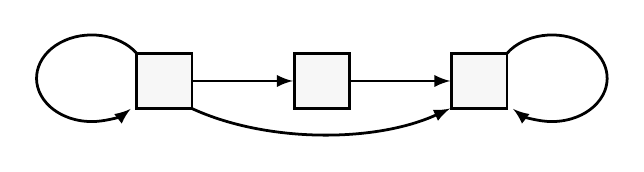
\begin{tikzpicture}
 [line width=1pt, bend angle=45,
 sq/.style={rectangle,inner sep=3pt, minimum size=7mm,
fill=black!3,draw=black}]
\node[sq] (dnode) at (0,0) {$\cchard$};
\node[sq] (fnode) at (2,0) {$\ccharf$};
\node[sq] (bnode) at (4,0) {$\ccharb$};
\draw[-latex] (dnode) -- (fnode);
\draw[-latex] (fnode) -- (bnode);
\draw[-latex] (-0.35,  0.35) arc(35:315:0.7cm and 0.55cm);
\draw[-latex] ( 4.35,  0.35) arc(145:-135:0.7cm and 0.55cm);
\draw[-latex] ( 0.35, -0.35) arc(230:310:2.55cm and 1.4cm);
\end{tikzpicture}\end{center}
% \caption{Transitions between types of values from the root of a tree in a filesystem}\label{fig_transition}
% \end{figure}

In this paper, $\FS$ and $\GS$ denote filesystems,
and $n$, $m$ and $o$ are nodes in $\setn$.
We write $\valf$ for an arbitrary file value. % element in $\setf$.

